\documentclass[tikz]{standalone}
\usetikzlibrary{calc}

\begin{document}
\begin{tikzpicture}[scale=1.2, transform shape]
  %\fill[black!80] (0,-3) rectangle (10,3);
  %\draw[help lines] (0,-3) grid (10,3);
  \coordinate (sun) at (1,0);
  \coordinate (sunt) at ($ (sun)+(0,1) $);
  \coordinate (sunb) at ($ (sun)-(0,1) $);
  \coordinate (moonp) at (7,0);

  \node[inner sep=0pt, outer sep=0pt] (moon) at (moonp) {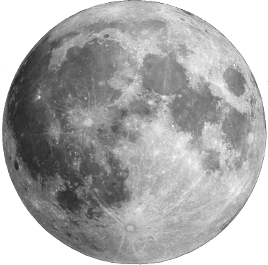
\includegraphics[width=0.6cm]{ch2_moon_small2.png}};

  \fill[yellow!50!orange, opacity=0.5] (sunt) -- (moon.north) -- (moon.south) -- (sunb) --cycle;
  \fill[yellow!50!orange, opacity=0.5] (sunt) -- (moon.south) -- (moon.north) -- (sunb) --cycle;
  %\fill[black!50] (8,-.9) -- ++(0,1.7) -- ++(1.5,.5) -- ++(0,-2.5) -- cycle;
  \node[rotate=23] at (10.3,0) {\includegraphics[width=3cm]{world.png}};
  \shade[inner color=yellow, outer color=orange] (1,0) circle (1cm);
  \coordinate (pernumbrat) at ($(moon.north)!-2cm!(sunb)$);
  \coordinate (pernumbrab) at ($(moon.south)!-2cm!(sunt)$);
  \coordinate (umbrat) at ($(moon.north)!-2cm!(sunt)$);
  \coordinate (umbrab) at ($(moon.south)!-2cm!(sunb)$);
  %\draw (sunb) +(14:8) coordinate (pernumbrat);
  %\draw (sunt) +(-14:8) coordinate (pernumbrab);
  %\draw (sunb) +(4.76:7.75) coordinate (umbrab);
  %\draw (sunt) +(-4.76:7.75) coordinate (umbrat);
  %\fill[black!60] let \p1=(pernumbrat) in (\x1,0) ellipse (5mm and \y1);
  \fill[black!70, opacity=0.5] let \p1=(umbrat) in (\x1,0) ellipse (0.5mm and \y1);
  \fill[black!95, opacity=0.5] (moon.north) -- (pernumbrat) to[out=0, in=0] (pernumbrab) -- (moon.south) -- cycle;
  \fill[black!95, opacity=0.5] (moon.north) -- (umbrat) to[out=0, in=0] (umbrab) -- (moon.south) -- cycle;
\end{tikzpicture}
\end{document}
